\documentclass[a4paper,12pt]{article}
\usepackage[margin=0.5in]{geometry}
\usepackage{hyperref}
\usepackage{subcaption}
\usepackage{tikz}
\usetikzlibrary{shapes,arrows}
\usetikzlibrary{decorations.pathreplacing}

\title{Regression Analysis in R}
\author{}
\date{}

\begin{document}

\vspace{-4em}

\maketitle

\vspace{-4em}

\section{Purpose}

The purpose of this activity is to provide you with an understanding of regression analysis (for the purposes of improving your understanding of Problem Sets 3 and 4, the quantitative reading material, and/or your final essay) and to both develop and apply that knowledge to the use of the R statistical programming environment.

\section{Overview}

This lab can be completed during at home and everything you need to know is provided in this document.

\section{Your Task}

Using R as instructed, complete the following activities.

\subsection{Bivariate Regression}

\begin{enumerate}
\item For this lab, we will use the UK portion of the European Social Survey (ESS) Round 7 data from 2014. You can download these data from here: \url{http://www.europeansocialsurvey.org/download.html?file=ESS6GB&c=GB&y=2014}. You may have to login with an email address and unzip the file. Save the file on your computer and unzip it.

\item Use \texttt{setwd()} to set your working directory to wherever you saved the file.

\item Read the data into R using: 

\begin{verbatim}
library("rio")
d <- import("ESS7GB.dta", haven = FALSE)
\end{verbatim}

\item How many observations are there in the dataset? How many variables?

\item Examine the \texttt{polintr} variable, which measures political interest. Tabulate the variable:

\begin{verbatim}
table(d$polintr)
\end{verbatim}

\noindent Then, replace the values of ``Refusal'', ``Don't know'', and ``No answer'' as missing values: 

\begin{verbatim}
levels(d$polintr)[5:7] <- NA
\end{verbatim}

\noindent Repeat the tabulation to confirm that this work. Using what you have learned already, attempt to answer the following questions:

\begin{enumerate}
\item What proportion respondents are ``very interested'' in politics?	
\item What is the \textit{modal} response category for this question?
\item What is the \textit{median} level of interest?
\item Using the gender variable (\texttt{gndr}), assess who is more interested in politics: men or women?
\item Using a statistical test, assess whether the difference in political interest is statistically distinguishable from zero.
\end{enumerate}

\item Now examine a different set of variables: happiness (\texttt{happy}) and religiosity (\texttt{rlgdgr}). First, remove the nonresponse categories from these variables:

\begin{verbatim}
levels(d$rlgdgr)[12:14] <- NA
levels(d$happy)[12:14] <- NA
\end{verbatim}

\item How happy are people in Great Britain on average? How religious are they?

\item Draw a scatterplot of religiosity and happiness:

\begin{verbatim}
library("ggplot2")
ggplot(d, aes(x = as.integer(rlgdgr), y = as.integer(happy))) +
    geom_jitter(na.rm = TRUE)
\end{verbatim}

\noindent Looking at the plot, how correlated would you say these variables are? Does happiness go with religiosity?

\item Use \texttt{cov()} to calculate the covariance of these two variables and \texttt{cor()} to calculate the correlation coefficient for this relationship. Note: You will have to wrap the variable names in \texttt{as.integer()} (like in the above code) in order to do these calculations. Also, see \texttt{? cor} and read about the \texttt{use} argument to \texttt{cor()} and \texttt{cov()} in order to correctly calculate these statistics.

\item Recall that the correlation is simply a rescaled version of the covariation: it is the covariance of two variables divided by the product of their standard deviations. Calculate the standard deviation of each variable and --- combined with the covariance you calculated above --- use that to manually calculate the correlation coefficient for this relationship. Does it match the value returned by \texttt{cor()}?

\item Recall that the correlation coefficient says nothing about the ``size'' of the relationship between two variables. Instead, it captures the degree to which that relationship is well-represented by a straight-line. If the correlation is high (close to -1 or +1), we know that the data can be well-represented by a line but we do not know how much of an increase we would expect to see in one variable given an increase in the other variable. ``Regression'' is a method for representing the covariance between variables in another way, which provides us with exactly this way of describing the relationship.

\item In regression, we draw a line through the scatterplot of the two variables that represents the ``line of best fit'' and that we can summarize by the ``slope'' of the line: the expected change in the y-axis variable given a one-unit increase in the x-axis variable. Add the following line to your scatterplot from above to see this line of best fit:

\begin{verbatim}
+ geom_smooth(method = "lm")
\end{verbatim}

\item To estimate the value of the slope, all we need to know is that the slope of the line is a rescaled version of the covariance of the two variables. Unlike the correlation coefficient, however, to estimate the slope, we rescale the covariance by the variance of the x-axis variable. To do this calculation, we have to be a little careful, so let's create a new data.frame to store our variables:

\begin{verbatim}
new <- na.omit(data.frame(religiosity = as.integer(d$rlgdgr),
                          happy = as.integer(d$happy)))
\end{verbatim}

\noindent Note: We use \texttt{na.omit()} here to remove missing data from these two variables. How many observations did we lose by removing these missing values?

\item Now, using the \texttt{new} data.frame, calculate the covariance of the two variables. Then, calculate the variance of \texttt{religiosity}. Divide the covariance by the variance of religiosity. This is the slope of the regression line. How much happier is someone if they were to increase their religiosity by one point on this question scale? Does this correspond with the relationship in your scatterplot; can you see the slope of the line matches this calculated slope?

\item We do not have to manually calculate the slope in this way. Indeed, R provides a function called \texttt{lm()} that allows us to calculate this directly. In R, run the following to estimate this regression model and store the results as an object called \texttt{m}. View the results.

\begin{verbatim}
m <- lm(happy ~ religiosity, data = new)
m
\end{verbatim}

\noindent Does the slope match what you calculated by hand?

\item Another way of thinking about regression is in terms of the ``sum of squares.'' We can think of the ``sum of squares'' as the total amount of variation in the y variable (happiness). You can calculate the total sum of squares for our data using:

\begin{verbatim}
sum((new$happy - mean(new$happy))^2)
\end{verbatim}

\noindent This quantity (the total sum of squares) is literally a sum of the area of several squares. Figure \ref{fig:tss}(a) shows this for a simple example scatterplot. The total sum of squares is simply the sum of the individual deviation of each observed value of y from the mean of y, squared.

\begin{figure}
    \centering
\begin{subfigure}[t]{0.49\columnwidth}
\centering
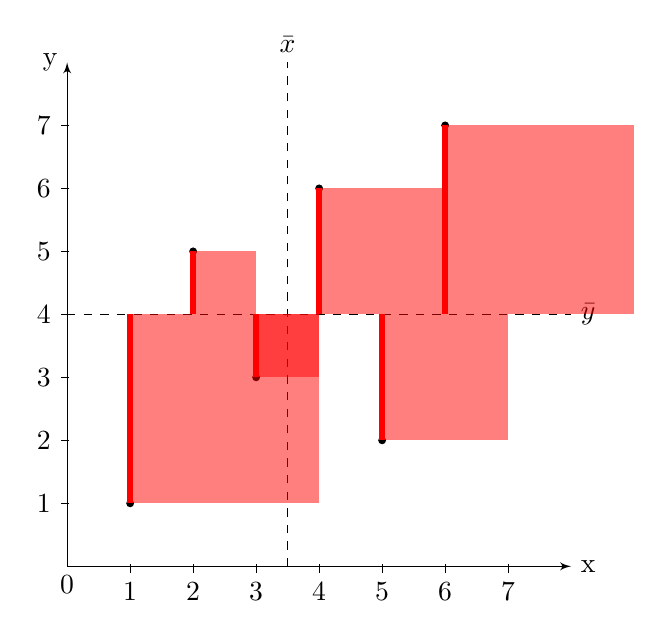
\begin{tikzpicture}[>=latex', scale=0.8]
\draw[->] (0,0) node[below] (origin) {0}  -- (8,0) node[right] (xaxis) {x};
\draw[->] (origin) -- (0,8) node[left] (yaxis) {y};
% x ticks
\foreach \x in {1,...,7}
    \draw (\x,1pt) -- (\x,-3pt) node[anchor=north] {$\x$};
% y ticks
\foreach \y in {1,...,7}
    \draw (1pt,\y) -- (-3pt,\y) node[anchor=east] {$\y$};
% points
\draw[fill] (1,1) circle [radius=1.5pt];
\draw[fill] (2,5) circle [radius=1.5pt];
\draw[fill] (3,3) circle [radius=1.5pt];
\draw[fill] (4,6) circle [radius=1.5pt];
\draw[fill] (5,2) circle [radius=1.5pt];
\draw[fill] (6,7) circle [radius=1.5pt];
% x-bar
\draw[dashed] (3.5, 0) -- (3.5,8) node[above] {$\bar{x}$};
% y-bar
\draw[dashed] (0,4) -- (8,4) node[right] {$\bar{y}$};

% x-deviations
%\draw[red, line width=2pt] (1,1) -- (3.5,1);
%\draw[red, line width=2pt] (2,5) -- (3.5,5);
%\draw[red, line width=2pt] (3,3) -- (3.5,3);
%\draw[red, line width=2pt] (4,6) -- (3.5,6);
%\draw[red, line width=2pt] (5,2) -- (3.5,2);
%\draw[red, line width=2pt] (6,7) -- (3.5,7);
% y-deviations
\draw[red, line width=2pt] (1,1) -- (1,4);
\draw[red, line width=2pt] (2,5) -- (2,4);
\draw[red, line width=2pt] (3,3) -- (3,4);
\draw[red, line width=2pt] (4,6) -- (4,4);
\draw[red, line width=2pt] (5,2) -- (5,4);
\draw[red, line width=2pt] (6,7) -- (6,4);

\fill[red, opacity=0.5] (1,1) rectangle (4,4);
\fill[red, opacity=0.5] (2,5) rectangle (3,4);
\fill[red, opacity=0.5] (3,3) rectangle (4,4);
\fill[red, opacity=0.5] (4,6) rectangle (6,4);
\fill[red, opacity=0.5] (5,2) rectangle (7,4);
\fill[red, opacity=0.5] (6,7) rectangle (9,4);

% line
%\draw[blue, line width=2pt] (0,1.6) -- (8,7.0856);

% residuals
%\draw[blue, line width=1pt] (1,1) -- (1,2.29);
%\draw[blue, line width=1pt] (2,5) -- (2,2.97);
%\draw[blue, line width=1pt] (3,3) -- (3,3.66);
%\draw[blue, line width=1pt] (4,6) -- (4,4.34);
%\draw[blue, line width=1pt] (5,2) -- (5,5.03);
%\draw[blue, line width=1pt] (6,7) -- (6,5.71);

%\fill[blue, opacity=0.5] (1,1) rectangle (2.29,2.29);
%\fill[blue, opacity=0.5] (2,5) rectangle (4.03,2.97);
%\fill[blue, opacity=0.5] (3,3) rectangle (3.66,3.66);
%\fill[blue, opacity=0.5] (4,6) rectangle (5.66,4.34);
%\fill[blue, opacity=0.5] (5,2) rectangle (8.03,5.03);
%\fill[blue, opacity=0.5] (6,7) rectangle (7.29,5.71);
\end{tikzpicture}
\caption{Total Sum of Squares}
\end{subfigure}
\begin{subfigure}[t]{0.49\columnwidth}
\centering
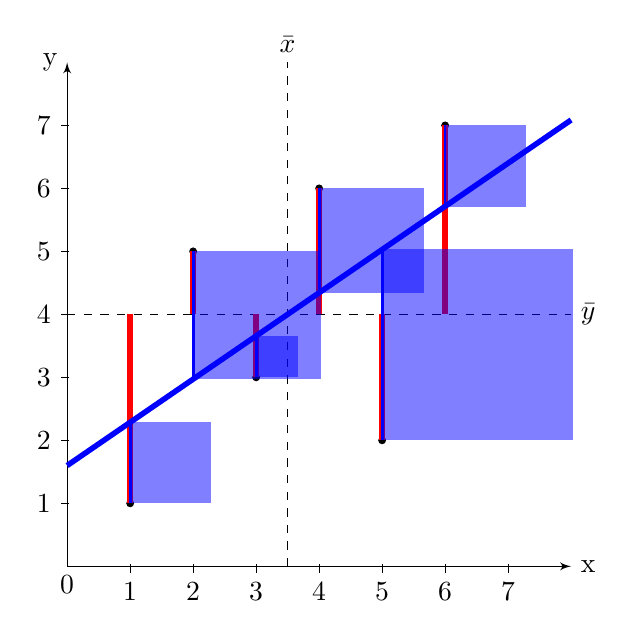
\begin{tikzpicture}[>=latex', scale=0.8]
\draw[->] (0,0) node[below] (origin) {0}  -- (8,0) node[right] (xaxis) {x};
\draw[->] (origin) -- (0,8) node[left] (yaxis) {y};
% x ticks
\foreach \x in {1,...,7}
    \draw (\x,1pt) -- (\x,-3pt) node[anchor=north] {$\x$};
% y ticks
\foreach \y in {1,...,7}
    \draw (1pt,\y) -- (-3pt,\y) node[anchor=east] {$\y$};
% points
\draw[fill] (1,1) circle [radius=1.5pt];
\draw[fill] (2,5) circle [radius=1.5pt];
\draw[fill] (3,3) circle [radius=1.5pt];
\draw[fill] (4,6) circle [radius=1.5pt];
\draw[fill] (5,2) circle [radius=1.5pt];
\draw[fill] (6,7) circle [radius=1.5pt];
% x-bar
\draw[dashed] (3.5, 0) -- (3.5,8) node[above] {$\bar{x}$};
% y-bar
\draw[dashed] (0,4) -- (8,4) node[right] {$\bar{y}$};

% x-deviations
%\draw[red, line width=2pt] (1,1) -- (3.5,1);
%\draw[red, line width=2pt] (2,5) -- (3.5,5);
%\draw[red, line width=2pt] (3,3) -- (3.5,3);
%\draw[red, line width=2pt] (4,6) -- (3.5,6);
%\draw[red, line width=2pt] (5,2) -- (3.5,2);
%\draw[red, line width=2pt] (6,7) -- (3.5,7);
% y-deviations
\draw[red, line width=2pt] (1,1) -- (1,4);
\draw[red, line width=2pt] (2,5) -- (2,4);
\draw[red, line width=2pt] (3,3) -- (3,4);
\draw[red, line width=2pt] (4,6) -- (4,4);
\draw[red, line width=2pt] (5,2) -- (5,4);
\draw[red, line width=2pt] (6,7) -- (6,4);

%\fill[red, opacity=0.5] (1,1) rectangle (4,4);
%\fill[red, opacity=0.5] (2,5) rectangle (3,4);
%\fill[red, opacity=0.5] (3,3) rectangle (4,4);
%\fill[red, opacity=0.5] (4,6) rectangle (6,4);
%\fill[red, opacity=0.5] (5,2) rectangle (7,4);
%\fill[red, opacity=0.5] (6,7) rectangle (9,4);

% line
\draw[blue, line width=2pt] (0,1.6) -- (8,7.0856);

% residuals
\draw[blue, line width=1pt] (1,1) -- (1,2.29);
\draw[blue, line width=1pt] (2,5) -- (2,2.97);
\draw[blue, line width=1pt] (3,3) -- (3,3.66);
\draw[blue, line width=1pt] (4,6) -- (4,4.34);
\draw[blue, line width=1pt] (5,2) -- (5,5.03);
\draw[blue, line width=1pt] (6,7) -- (6,5.71);

\fill[blue, opacity=0.5] (1,1) rectangle (2.29,2.29);
\fill[blue, opacity=0.5] (2,5) rectangle (4.03,2.97);
\fill[blue, opacity=0.5] (3,3) rectangle (3.66,3.66);
\fill[blue, opacity=0.5] (4,6) rectangle (5.66,4.34);
\fill[blue, opacity=0.5] (5,2) rectangle (8.03,5.03);
\fill[blue, opacity=0.5] (6,7) rectangle (7.29,5.71);
\end{tikzpicture}
\caption{Residual Sum of Squares}
\end{subfigure}
\caption{Sum of Squares for a Simple Scatterplot}\label{fig:tss}
\end{figure}

\item In regression, we are ``explaining'' some of that total variation in y with the covariation between x (religiosity) and y (happiness). This explained portion of the sum of squares is called the ``sum of squares, explained'' or ``model sum of squares''; the amount of variation in y that is not ``explained'' by x is called the ``residual sum of squares''. This residual sum of squares is literally the sum of the squared areas formed by the distance between each point and the ``predicted value'' (or ``fitted value'') of y expected by the regression line given that observation's value of x. Figure \ref{fig:tss}(b) shows the residual sum of squares for the same example scatterplot.

\item If all of the variation in y is explained by the variation in x, then the residual sum of squares will be \textit{small} while the explained sum of squares will be large. You can calculate the residual sum of squares using the following:

\begin{verbatim}
sum((new$happy - (coef(m)[1] + (coef(m)[2] * new$religiosity)))^2)
\end{verbatim}

\noindent How large is the residual sum of squares compared to the total sum of squares you calculated above?

\item A common way to assess the ``goodness of fit'' of a regression estimation is whether the explained sum of squares is large. The proportion of the total sum of squares that is ``explained'' by the model is called the ``R-squared'' statistic, sometimes called the ``coefficient of determination.'' It is simply 1 minus the ratio of the residual sum of squares to the total sum of squares. It is interpreted as a proportion: if it is 0, then religiosity explains \textit{none} of the variation in happiness; if it is 1, then religiosity explains \textit{all} of the variation in happiness. What is the R-squared for this relationship?

\item Recall from earlier that the regression slope is simply a scaled version of the covariance of the two variables. The correlation coefficient is also a scaled version of the covariance. Now, you can also note that there is a direct correspondence between the correlation coefficient and the R-squared value you just calculated. R-squared is simply the bivariate correlation coefficient, squared. Try it and confirm this is the case.

\item This focus on the residuals allows us to demonstrate a few R programming features that have useful practical applications:

\begin{enumerate}
\item \texttt{m\$fitted} will return a vector containing the ``fitted value'' of y for each observation (given its value of x)
\item \texttt{m\$residuals} will return a vector containing the residuals for each observation in your dataset. These residuals will be equal to \texttt{new\$happy - m\$fitted}
\item The \texttt{predict()} function allows you to calculate the fitted value of y for a given value of x. By default, it simply returns the same thing as doing \texttt{all.equal(predict(m), m\$fitted)}. But, if you supply a data.frame as the value of the \texttt{newdata} argument, you can obtained the fitted value for an arbitrary value of x: \texttt{predict(m, newdata = data.frame(religiosity = 3))}
\end{enumerate}

\item Returning to our main focus, another common measure of model fit is called the residual mean squared error, or sometimes simply $\hat{\sigma}$. This is simply the standard deviation of the residuals (the unexplained variation in y). As religiosity explains more and more of the variation in happiness, then the residuals will become small and have a lower variance (and lower standard deviation).\footnote{Recall the standard deviation is simply the square root of the variance.} There are three ways to calculate sigma: (a) by manually calculating the residuals and taking the standard deviation thereof, (b) extracting the residuals from the \texttt{m} object (returned by \texttt{lm()}), or (c) using R's calculation of sigma:

\begin{verbatim}
sqrt(sum((new$happy - (coef(m)[1] + (coef(m)[2] * new$religiosity)))^2)/nrow(new))
sd(residuals(m))
\end{verbatim}

\noindent The reason this quantity is useful as a measure of model fit is that it is on the scale of the y-axis variable (happiness) and can be directly compared to the standard deviation of y. If religiosity explained a lot of the variation in happiness, then $\hat{\sigma}$ would be small compared to \texttt{sd(new\$happy)}. Is it?

\item Returning to our estimated regression model, \texttt{m}, use \texttt{summary(m)} to see a more complete print out of the regression results. Can you make sense of all of the information that is displayed? What are the values of the following quantities:

\begin{enumerate}
\item Regression slope
\item $\hat{\sigma}$
\item R-squared
\item Mean residual
\item y-intercept (the value of happiness when religiosity = 0)
\end{enumerate}

\item You will note that the table includes a number of other statistics that we haven't discussed, including the standard errors of the regression slope and y-intercept, and t-statistics and p-values for each of these. We are not going to cover the calculation of the standard errors, but can you see how the t-statistics are calculated given what we covered last week?

\item Is the estimated regression slope substantively large? Is the slope significantly different from zero?

\item In order to ensure your understanding, you may want to redo some of these exercises using other combinations of variables (e.g., political interest, etc.). One particularly illustrative example would be to use gender as an x-axis variable. (You will want to redefine \texttt{gender} as:

\begin{verbatim}
d$gender <- as.integer(d$gndr)-1
\end{verbatim}

\noindent In that case, you will hopefully note some similarities between the conditional mean of an outcome variable given gender:

\begin{verbatim}
aggregate(as.integer(polintr) ~ gender, data = d, FUN = mean, na.rm = TRUE)
\end{verbatim}

\noindent and the results of a corresponding regression analysis:

\begin{verbatim}
lm(as.integer(polintr) ~ gender, data = d)
\end{verbatim}

\item Recall that the p-value in a statistical significance test represents the probability of observing a t-statistic as large or larger than the one observed in a sample of the data from a population where the true t-statistic is zero (in this case, where the slope of the relationship between religiosity and happiness is non-existent).

As an \textbf{advanced exercise}, you emulate that process of repeated sampling through a process known as ``bootstrapping''. In bootstrapping, you treat your sample data as if they were a population and draw repeated samples (with replacement) from your sample and apply an estimator (in this case, a regression estimator) to each resampled dataset. In essence, bootstrapping creates an approximate sampling distribution for your statistic.

If you extract the estimated slope from each bootstrap sample, this bootstrap sampling distribution mimics the hypothetical distribution of slopes you would expect to observe in a population where the true slope was equal to that observed in your actual sample data. The proportion of slopes less than zero in this bootstrapped distribution can be interpreted as the p-value (the probability of observing a slope as large as the one you observed) from a population where the true slope was zero.

Here's the code:

\begin{verbatim}
boot <- replicate(5000L, 
          lm(happy ~ religiosity, 
             data = new[sample(1:nrow(new), nrow(new), TRUE), ])$coef[2])
summary(boot)
sum(boot < 0)/length(boot) # p-value
\end{verbatim}

\noindent What is p-value of the regression slope, based on the bootstrap sampling distribution?

\end{enumerate}

\subsection{Multivariate Regression}

\begin{enumerate}

\item Think again about political interest. How correlated are interest, happiness, gender, and religiosity? If they are correlated, can we interpret those correlations as causal relationships? What criteria for causal inference to we have to satisfy in order to interpret this correlation as a causal relationship?

\item One major barrier to causal inference here is confounding: the relationship between these two factors may be explained by some other variable or variables. We might be concerned that there is some earlier variable, that precedes both religiosity and (current) happiness in time that causes both variables, and in turn makes it appear that the two variables are related due to a causal relationship between religiosity and happiness.

To think about this possibility, it can be useful to draw a ``causal diagram'' in the form of a ``directed, acyclic graph'' (DAG). Figure \ref{fig:causalgraph} shows an example DAG. We can imagine that religiosity is \textbf{X} and happiness is \textbf{Y}. We are concerned bout variables like \textbf{Z} and \textbf{W} that cause both. Draw a possible DAG, labeling possible confounding variables. (You might also want to include other variables in your graph, like \textbf{A} and \textbf{E} that cause happiness but that you do not think cause religiosity.)

\begin{figure}
\centering
\begin{tikzpicture}[>=latex',circ/.style={draw, shape=circle, node distance=5cm, line width=1.5pt}]
    \draw[->] (0,0) node[left] (X) {X} -- (2.5,0) node[right] (D) {D};
    \draw[->] (3.1,0) -- (5,0) node[right] (Y) {Y};
    \draw[->] (-3,3) node[above] (Z) {Z} -- (X);
    \draw[->] (Z) -- (Y);
    \draw[->] (5,2) node[above] (A) {A} -- (Y);
    \draw[->] (4,-2) node[below] (E) {E} -- (Y);
    \draw[->] (X) -- (1,-0.5) node[right] (C) {C};
    \draw[->] (-2, -2) node[below] (W) {W} -- (X);
    \draw[->] (-3,-1) node[above] (B) {B} -- (W);
    \draw[->] (W) -- (Y);
\end{tikzpicture}
\caption{A Causal Graph}\label{fig:causalgraph}
\end{figure}


\item Once you have a reasonable DAG showing possibly causal relationships, think about whether you can observe any of the variables in your DAG. Are all of the potentially confounding variables you named available in the ESS dataset? You can find a complete listing of variables in: \texttt{attributes(d)\$var.labels} or in the complete documentation of the ESS questionnaire here: \url{http://www.europeansocialsurvey.org/docs/round7/fieldwork/united_kingdom/ESS7_questionnaires_GB.pdf}.

\item If you have access to potentially confounding variables, then we can use an elaboration of the bivariate regression models we just discussed to help to control for this confounding. If potentially confounding variables in your DAG are unobserved (either because they are not included in the ESS or because they are perhaps ``unobservable'' factors), there is nothing we can do to rule out the potential for confounding. We are, in that situation, completely unable to draw a causal inference from the observational data in front of us. We would need more data!

\item How can multiple regression help us to address confounding? The mathematics here is a bit complicated, but the following exercises are meant to provide some intuition. Before we begin, make sure you have a firm grasp on the variables you have identified. Use \texttt{summary()} or other functions to know the key statistics of each variable and \texttt{ggplot2} to produce scatterplots or other graphics comparing these variables to one another.

\item Multiple regression works by simultaneously accounting for the influence of multiple ``right hand side'' (RHS) variables on a single ``outcome'' variable (\textbf{Y} in the example DAG in Figure \ref{fig:causalgraph}). How does it do this? Let's start with a simple example (which you can expand using the variables in your DAG). In the below model we are trying to see whether there is still an association between religiosity and happiness once we ``control for'' interest in politics:

\begin{verbatim}
new2 <- na.omit(data.frame(happy = as.integer(d$happy),
                  religiosity = as.integer(d$rlgdgr),
                  pinterest = as.integer(d$polintr),
                  gender = as.integer(d$gndr)))
m2 <- lm(happy ~ religiosity + pinterest, data = new2)
\end{verbatim}

\noindent Basically, this model says that we think happiness might be a function of religiosity, political interest, and gender, and we want to know how much each contributes to happiness. By including all variable in one regression equation, we estimate the influence of each variable on the outcome accounting for the simultaneous influence of the other RHS variables. Is there still a relationship between religiosity and happiness once we account for these other factors?

\item Try estimating bivariate relationships between each of these RHS variables and the outcome. How do the estimated slopes in the bivariate models compare to the estimated slopes in the multivariate specification?

\begin{verbatim}
p1 <- lm(happy ~ religiosity, data = new2)
p2 <- lm(happy ~ pinterest, data = new2)
\end{verbatim}

\item When we regress an outcome on a variable, we aim to \textit{break} the correlation between the residuals (the unexplained parts of y) and the RHS variable. TO see this, look at the correlations between the residuals from each of the bivariate models and the RHS variable we included:

\begin{verbatim}
cor(p1$residuals, new2$religiosity)
cor(p2$residuals, new2$pinterest)
\end{verbatim}

\noindent This correlation is basically zero in each case.

\item But when we exclude a RHS variable (leaving it out of the regression equation), the residuals of y might still be associated with that variable:

\begin{verbatim}
round(cor(cbind(p1$residuals, new2$religiosity, new2$pinterest)), 3)
round(cor(cbind(p2$residuals, new2$religiosity, new2$pinterest)), 3)
\end{verbatim}

\item We can see that the excluded variables appear to still be associated with the outcome (i.e., there is some residual some of squares that is still associated with the excluded RHS variables). If we include these, as in the multivariate model \texttt{m2}, we can account for the independent influences of each of these factors. But how does this work? To understand multiple regression we have to understand a simpler concept: the \textit{partial correlation}.

A partial correlation is the correlation between two variables controlling for the influence of a third variable. If we want to know the partial correlation between \texttt{happy} and \texttt{religiosity}, controlling for \texttt{pinterest}, we regress each variable on \texttt{pinterest} and correlate their residuals:

\begin{verbatim}
r1 <- lm(happy ~ pinterest, data = new2)$residuals
r2 <- lm(religiosity ~ pinterest, data = new2)$residuals
cor(r1, r2)
\end{verbatim}

\noindent This removes the common influence of the third variable from the original correlation:

\begin{verbatim}
cor(new2$happy, new2$religiosity)
\end{verbatim}

\noindent which in this case is small.

\item Multiple regression is simply a series of partial correlations. If we want to know the slope of the relationship between religiosity and happiness, we simply regress the residuals of the regression of \texttt{happy} on \texttt{pintrest} on the residuals from the regression of \texttt{religiosity} on \texttt{pinterest}:

\begin{verbatim}
lm(r1 ~ r2)
# or:
lm( lm(happy ~ pinterest, data = new2)$residuals ~
    lm(religiosity ~ pinterest, data = new2)$residuals )$coef
\end{verbatim}

\noindent Similarly, if we want to know the influence of political interest controlling for religiosity, we do something analogous:

\begin{verbatim}
lm( lm(happy ~ religiosity, data = new2)$residuals ~
    lm(pinterest ~ religiosity, data = new2)$residuals )$coef
\end{verbatim}

\noindent Note how the slope for \texttt{pinterest} and the slope for \texttt{religiosity} in the previous two partial correlation models are identical to the slopes from a multivariate regression of \texttt{happy} on both \texttt{pinterest} and \texttt{religiosity}:

\begin{verbatim}
lm(happy ~ pinterest + religiosity, data = new2)$coef
\end{verbatim}

\noindent All a multiple regression model is doing is engaging a series of simultaneous regressions of the outcome on each RHS variable and each RHS variable on all the other RHS variables.

\item Everything that we learned above about bivariate regressions --- residuals, fitted/predicted values, measures of model fit, statistical significance, etc. --- applies in a multiple regression context. Explore some of these aspects of the multivariate regression models we have just estimated.

\item The only thing that is different about bivariate and multivariate regression is the substantive interpretation of estimated regression slopes. Rather than talk about these slopes as the ``influence of X on Y'' we instead interpret them as the ``influence of X on Y controlling for Z'' or the ``influence of X on Y all else constant''. This is a subtle change but it's important to remember that in a multivariate regression we are not estimating a \textit{raw} relationship but rather than relationship accounting for the variance in X and Y explained by the other RHS variables in the model. For this reason, the slopes in a multivariate regression are sometimes called ``marginal effects'' due to their representing the change of influence of one variable while the other variables remain constant.

\end{enumerate}


\end{document}


